\documentclass[article]{jlreq}
\usepackage[dvipdfmx]{graphicx}
\usepackage{here}
\usepackage{amsmath}
\usepackage{latexsym}
\usepackage{multirow}
\usepackage{textcomp}
\usepackage{url}
\usepackage{array}    % 列の設定
\usepackage{caption}
\usepackage{booktabs}
\usepackage[utf8]{inputenc}
\usepackage{subcaption}
\newcommand{\ita}{\textit}
\newcommand{\ko}{\rm{k$\Omega$}}
\newcommand{\om}{\rm$\Omega$}
\newcommand{\nf}{\rm{nF}}
\title{}
\date{}
\begin{document}\maketitle




以下に今回用いた回路を示す。
\begin{figure}[H]
    \centering
    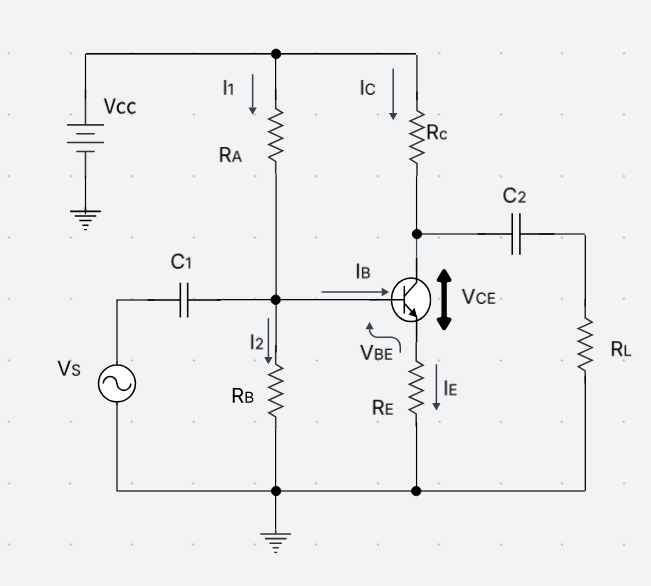
\includegraphics[scale=0.5]{kairozu3.png}
    \caption{実験で用いた回路}
\end{figure}

\section{実験1}
\subsection{実験内容}
与えられたトランジスタの静特性(図2)を用いて,$V_{CC} = 16\,\text{V}, R_{C} = 3\,\text{k}\Omega , R_{E} = 1\,\text{k}\Omega $として,動作点を負荷直線の
中心部に設定し,$R_A,R_B$ を求めた。
\begin{figure}[H]
    \centering
    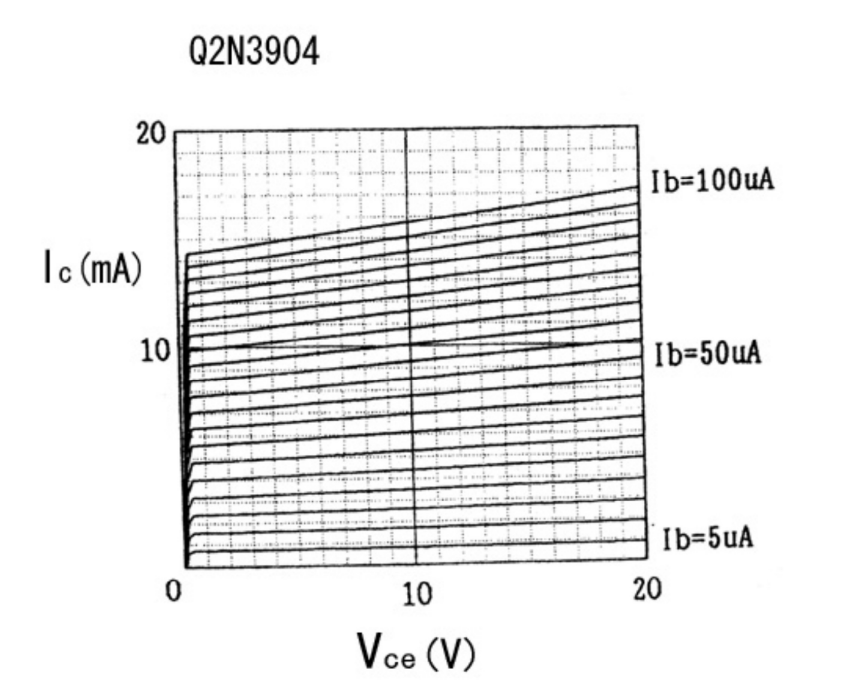
\includegraphics[scale=0.5]{hukatyokusenn0.png}
    \caption{トランジスタの静特性}
\end{figure}

\subsection{結果}
図1から$I_B$と$I_C$の和が$I_E$という関係から以下の式が成り立つ。
ただし、$\beta = \frac{I_C}{I_B}$は電流増幅率を表し、$\frac{1}{\beta}$
は0に近似できるとする。
\begin{align}
I_E &= I_B + I_C \notag \\
    &= \left(1+\frac{1}{\beta}\right) I_C \notag \\
    &\simeq I_C
\end{align}
また
\begin{align}
V_{CC} &= R_CI_C + V_{CE} + R_EI_E \notag \\
    &\simeq (R_C + R_E)I_C + V_{CE} 
\end{align}
より、$I_C$は
\begin{align}
    I_C &= -\frac{V_{CE}}{R_C + R_E} + \frac{V_{CC}}{R_C + R_E} \notag \\
        &= -\frac{V_{CE}}{3 + 1} + \frac{16}{3 + 1} \notag \\
        &= -\frac{V_{CE}}{4} + 4\,[\mathrm{mA}]
\end{align}
となる。これを負荷直線として図2に加えると以下のようになる。
\begin{figure}[H]
    \centering
    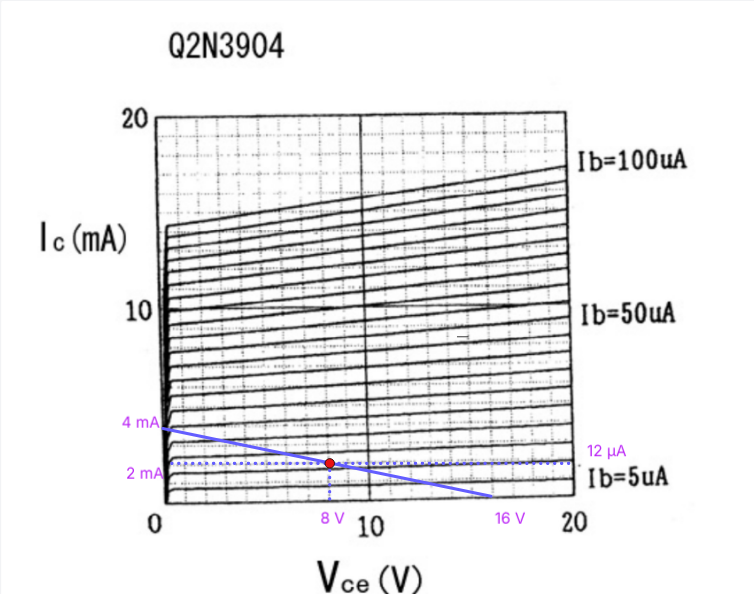
\includegraphics[scale=0.5]{hukatyokusenn.png}
    \caption{負荷直線}
\end{figure}
よって、負荷直線の中心部を$8\,\mathrm{V}$と設定できる。
また，$I_E \simeq I_C$ より，
\begin{align}
V_B
&= V_{BE}+R_E I_E \notag \\
&\simeq V_{BE}+R_E I_C
\end{align}

さらに，
\begin{align}
I_1 &= 20 I_{BP} \\
I_2 &= I_1 - I_{BP} \notag \\
    &= 19 I_{BP}
\end{align}

したがって，
\begin{align}
R_B
&= \frac{V_B}{I_2} \notag \\
&= \frac{V_{BE}+R_E I_C}{19 I_{BP}}
\end{align}

また，
\begin{align}
R_A
&= \frac{V_{CC}-V_B}{I_1} \notag \\
&= \frac{V_{CC}-(V_{BE}+R_E I_C)}{20 I_{BP}}
\end{align}


ここで、図3から、$I_{CP}=2\,\mathrm{mA},\quad I_{BP}=12\,\mu\mathrm{A}$であることが分かる。
また、$V_{BE}$ は一般に $0.6\sim0.7\,\mathrm{V}$ 程度であるため，
その中間値として $V_{BE}=0.65\,\mathrm{V}$ とする。
以上より

\[
R_A \approx 55.625\,\mathrm{k\Omega},\quad
R_B \approx 11.623\,\mathrm{k\Omega}
\]
と求まる。

\subsection{考察}
本実験では，動作点を負荷直線の中央付近に設定した。
これは，入力信号により電流および電圧が動作点を中心として増減する際に，
上下方向に対して対称な変化が可能となり，
出力波形の歪みを抑えることができるためである。


\section{実験2}
\subsection{実験内容}
実験1で求めた抵抗値を使い、
$C_{1} = C_{2} = 10\,\mu\mathrm{F},\; R_{L} = 1\,\mathrm{M}\Omega $としたときの
周波数特性（振幅特性および位相特性,$1\,\mathrm{Hz} \sim 100\,\mathrm{MHz}$）を求めた。
以下にLTspiceにより作成した回路図を示す。
\begin{figure}[H]
    \centering
    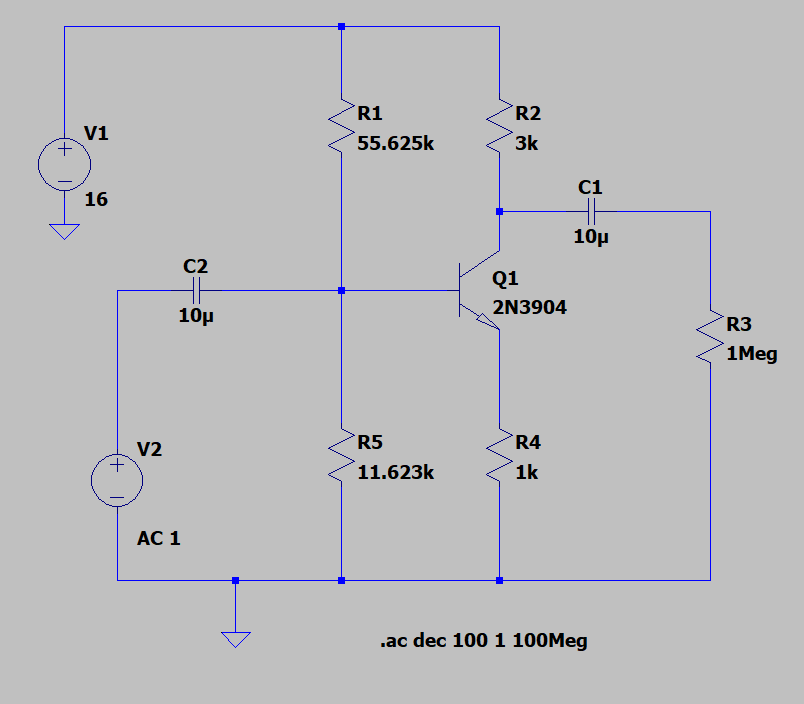
\includegraphics[scale=0.25]{kairozu3-2.png}
    \caption{}
\end{figure}
\subsection{結果}
以下に解析結果を示す。
\begin{figure}[H]
    \centering
    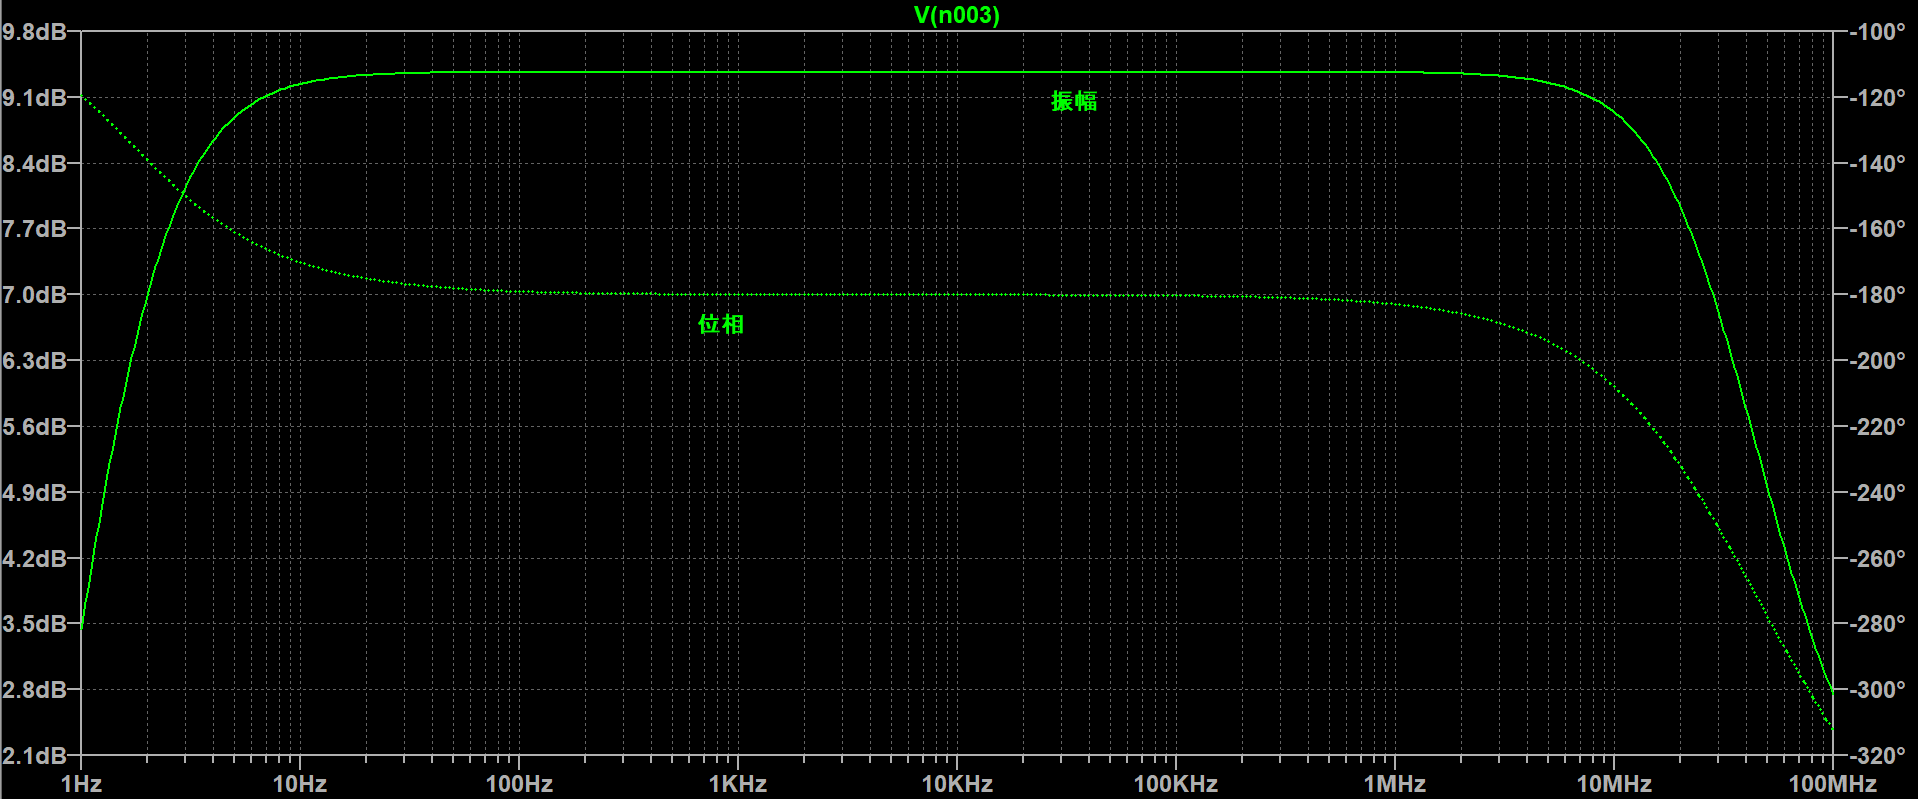
\includegraphics[scale=0.25]{ac3-2.png}
    \caption{}
\end{figure}
\subsection{考察}

まず，低周波領域では出力電圧が小さくなることが確認できる。
これは入力側および出力側に接続されたコンデンサ $C_1, C_2$ のインピーダンスが大きくなり，
信号が回路内に十分に伝わらないためであると考えられる。

次に，中間の周波数領域では入力電圧に対して出力電圧が大きくなり，
一定の増幅が得られていることが分かる。
解析結果より，中間領域における振幅特性は約 $9.36\,\mathrm{dB}$ であった。
これを電圧比に変換すると，
\[
20\log_{10}A_v = 9.36
\]
より，
\[
A_v = 10^{9.36/20} \approx 2.94
\]
となる。
したがって、本回路は入力電圧を約3倍に増幅しているといえる。

また、高周波領域では再び出力電圧が小さくなることが確認できる。
これは入力信号の変化が速くなることで、
回路がその変化に十分に追従できなくなり、
電圧の変化が出力まで伝わりにくくなるためであると考えられる。

さらに、位相特性より中間の周波数領域において入力と出力が反転していることが確認できる。
これは本回路がエミッタ接地回路であり、
入力信号に対して出力信号が反転する特性を持つためである。

\section{実験3}
\subsection{実験内容}
周波数 $f = 10\,\mathrm{kHz}$，振幅 $V_{\mathrm{AMP}} = 0.5\,\mathrm{V}$ の正弦波を入力したとき，
負荷抵抗 $R_{\mathrm{L}}$ の出力波形を求めた。
以下にLTspiceにより作成した回路図を示す。
\begin{figure}[H]
    \centering
    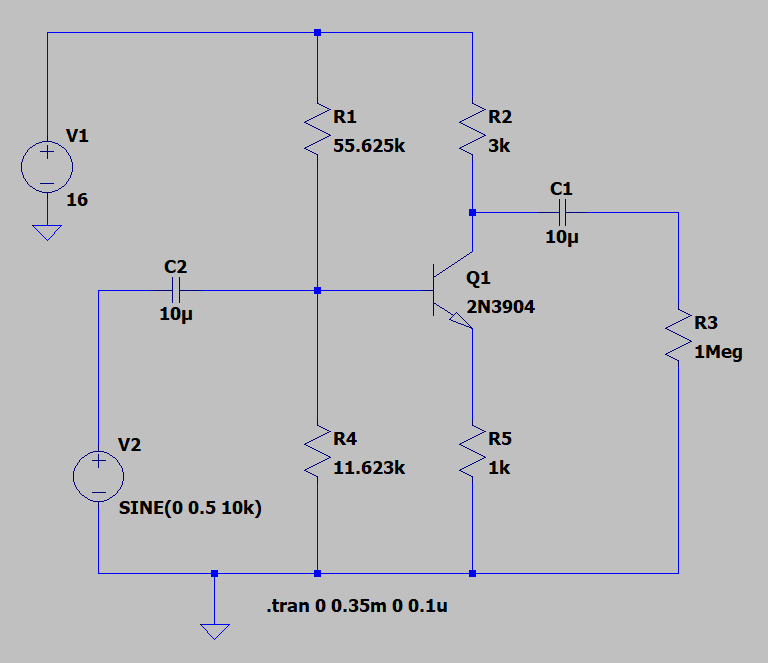
\includegraphics[scale=0.25]{kairozu3-31.png}
    \caption{}
\end{figure}

さらに，入力振幅 $V_{\mathrm{AMP}} = 0.5\,\mathrm{V}$ を徐々に大きくしていき，
出力がクリップ直前（無歪最大出力）となるとき(ここでは$V_{\mathrm{AMP}} = 1.97\,\mathrm{V}$とした)の波形を求めた。
以下にLTspiceにより作成した回路図を示す。
\begin{figure}[H]
    \centering
    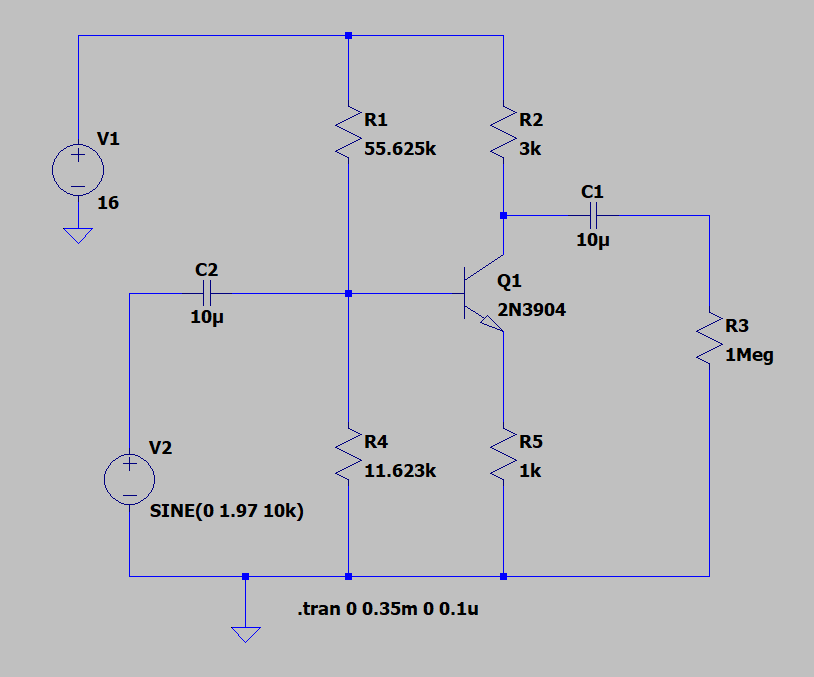
\includegraphics[scale=0.25]{kairozu3-32.png}
    \caption{}
\end{figure}

\subsection{結果}

\begin{figure}[H]
    \centering
    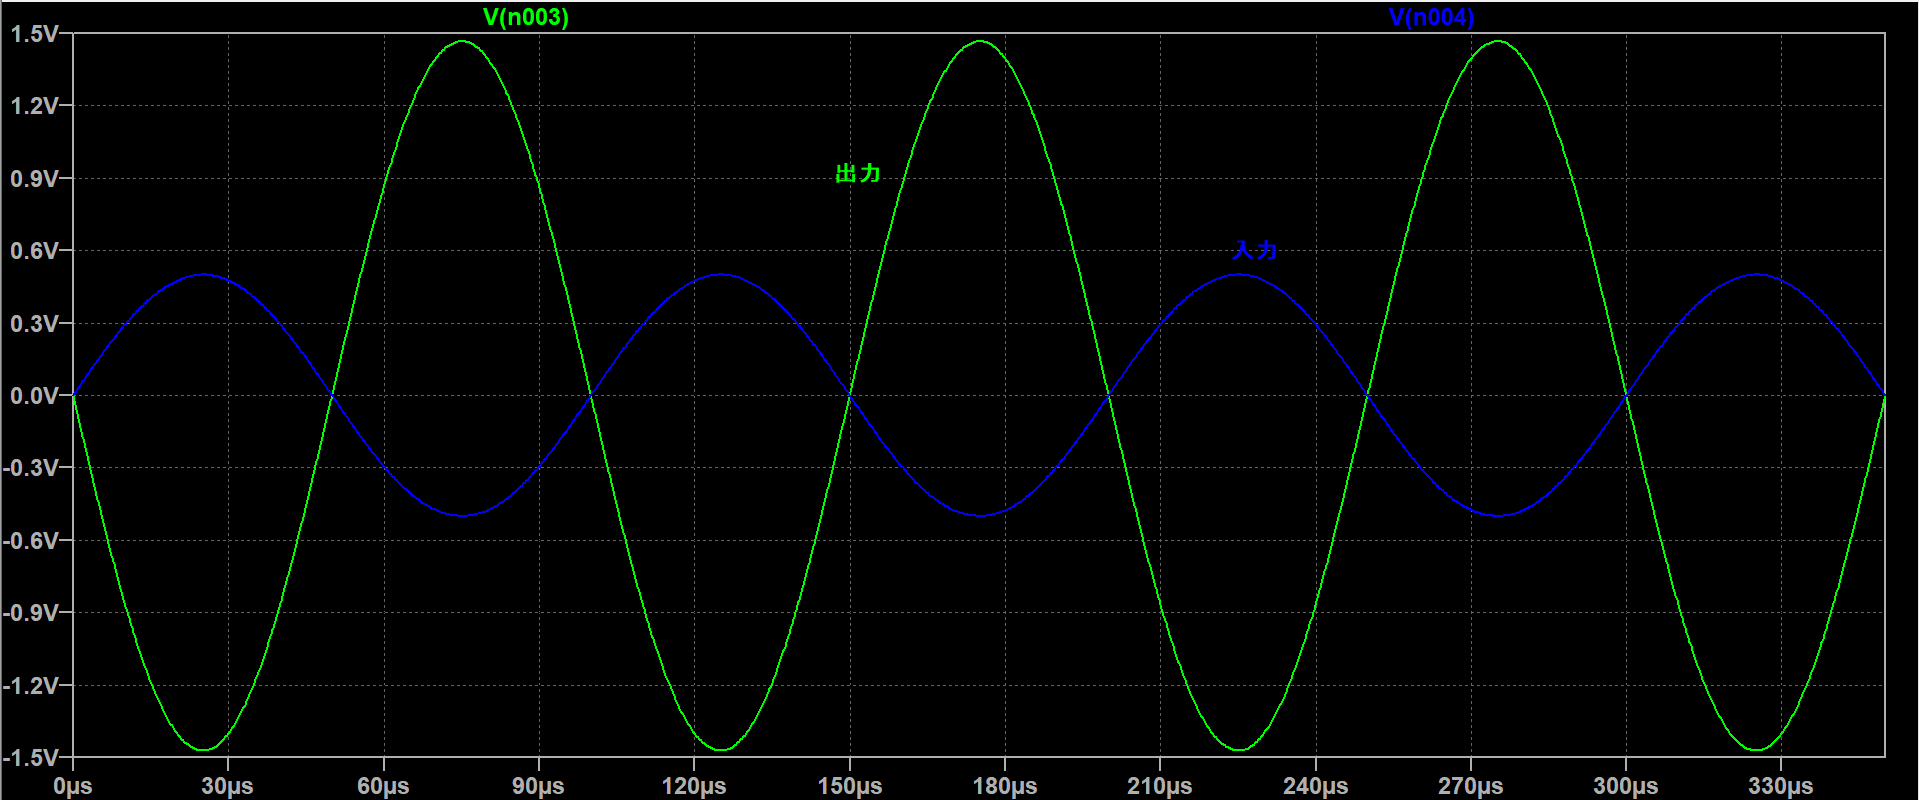
\includegraphics[scale=0.25]{sim3-31.png}
    \caption{$V_{\mathrm{AMP}} = 0.5\,\mathrm{V}$}
\end{figure}
\begin{figure}[H]
    \centering
    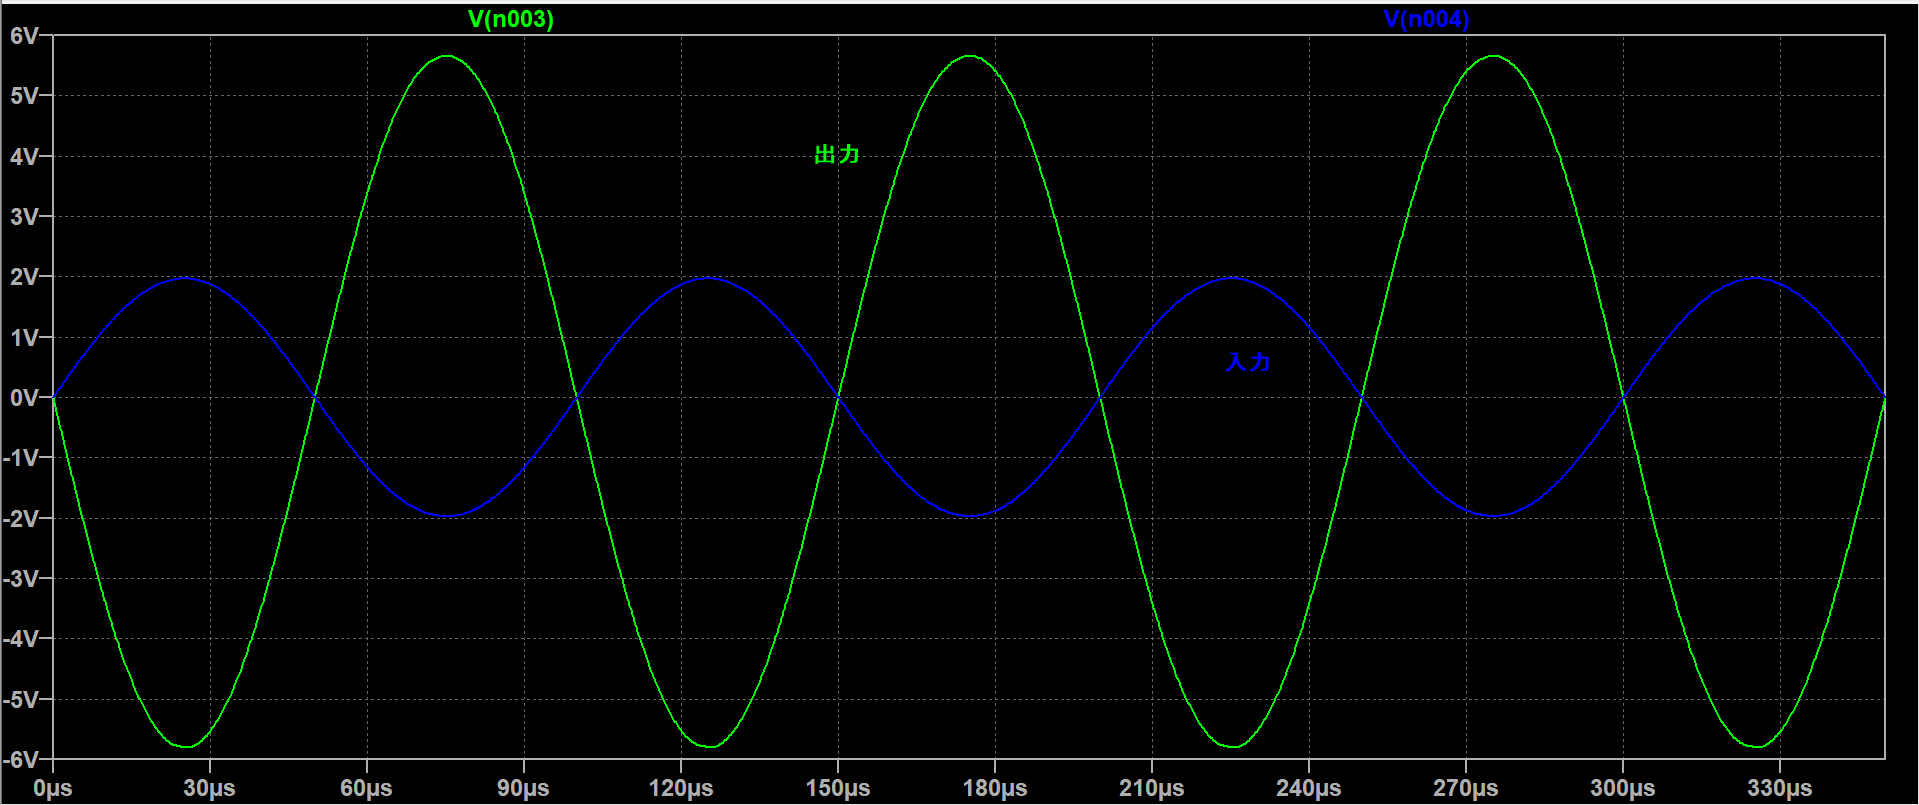
\includegraphics[scale=0.25]{sim3-32.png}
    \caption{$V_{\mathrm{AMP}} = 1.97\,\mathrm{V}$}
\end{figure}


\subsection{考察}
時間域解析において、
入力振幅 $0.5\,\mathrm{V}$ のときの出力振幅は約 $1.467\,\mathrm{V}$ であり、増幅率は
\[
\frac{1.467}{0.5} \approx 2.93
\]
となる。
また、入力振幅 $1.97\,\mathrm{V}$ のときの出力振幅は約 $5.65\,\mathrm{V}$ であり、増幅率は
\[
\frac{5.65}{1.97} \approx 2.87
\]
となった。

これより、小さい入力振幅の場合には、
入力電圧に対する出力電圧の比はほぼ一定であり、
周波数域解析で得られた値とよく一致していることが分かる。
一方、入力振幅を大きくすると、
出力電圧が回路の動作限界に近づくため、
増幅の割合がわずかに低下することが確認できる。

\section{実験4}
\subsection{実験内容}
実験3と同じ条件で解析し、コレクタとエミッタの電位の変化を観察した。
\subsection{結果}
以下にそれぞれの振幅における解析結果を示す。
ただし、紫色を入力波形、赤色を出力波形、青色をコレクタ電圧波形、黄色をエミッタ電圧波形
とする。
\begin{figure}[H]
    \centering
    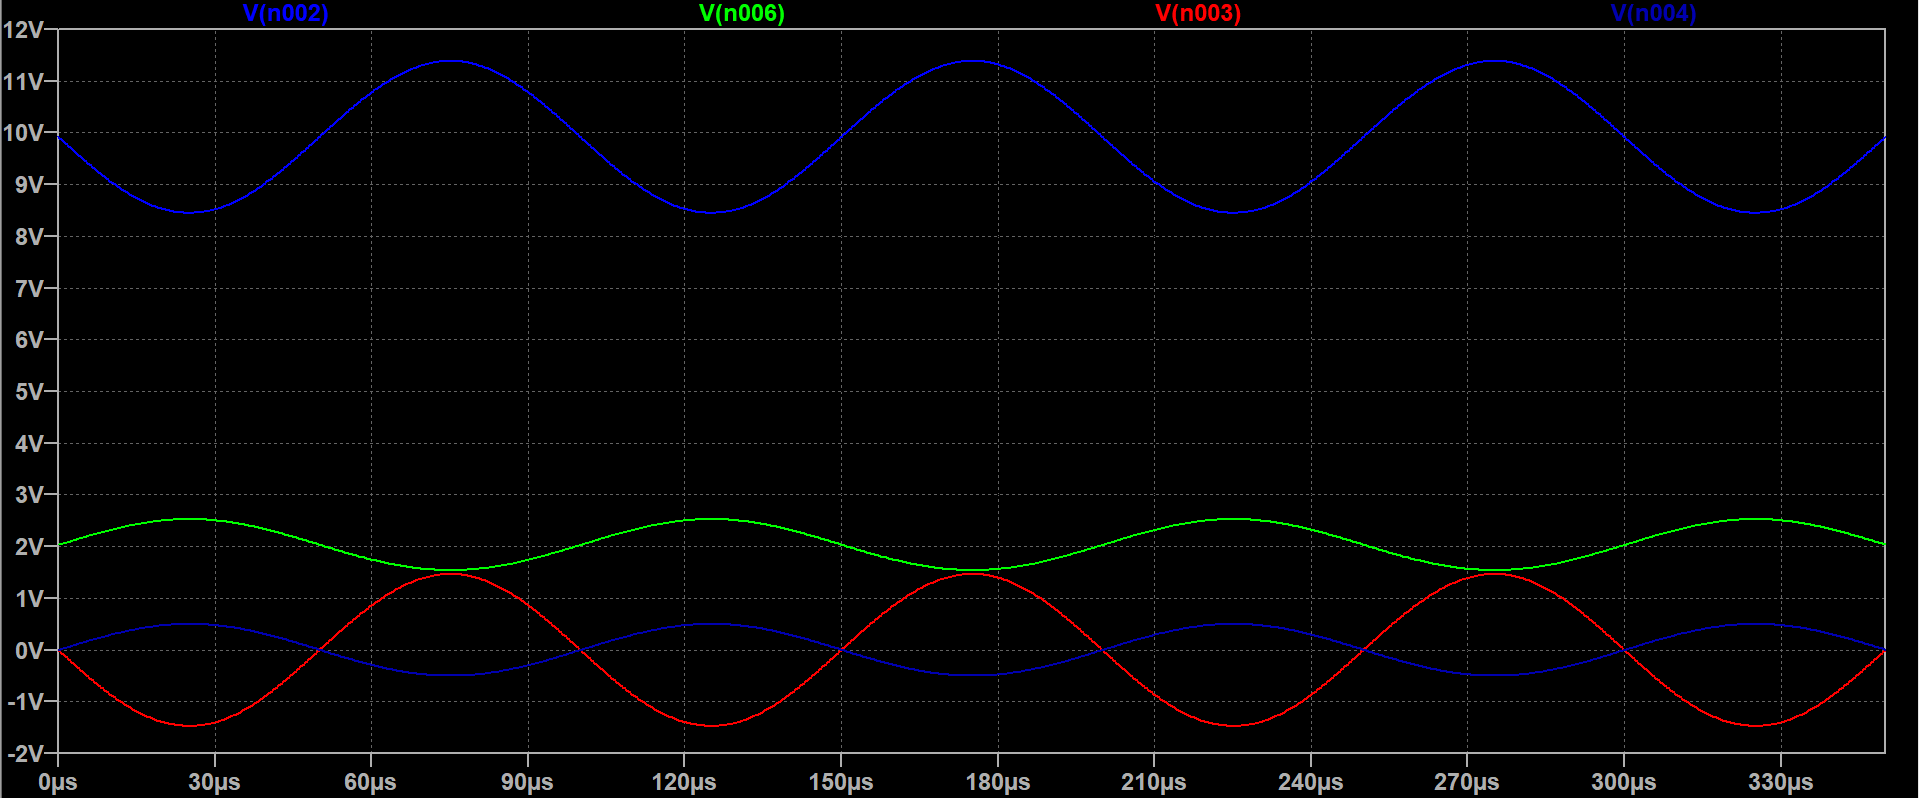
\includegraphics[scale=0.25]{sim4-1.png}
    \caption{$V_{\mathrm{AMP}} = 0.5\,\mathrm{V}$}
\end{figure}
\begin{figure}[H]
    \centering
    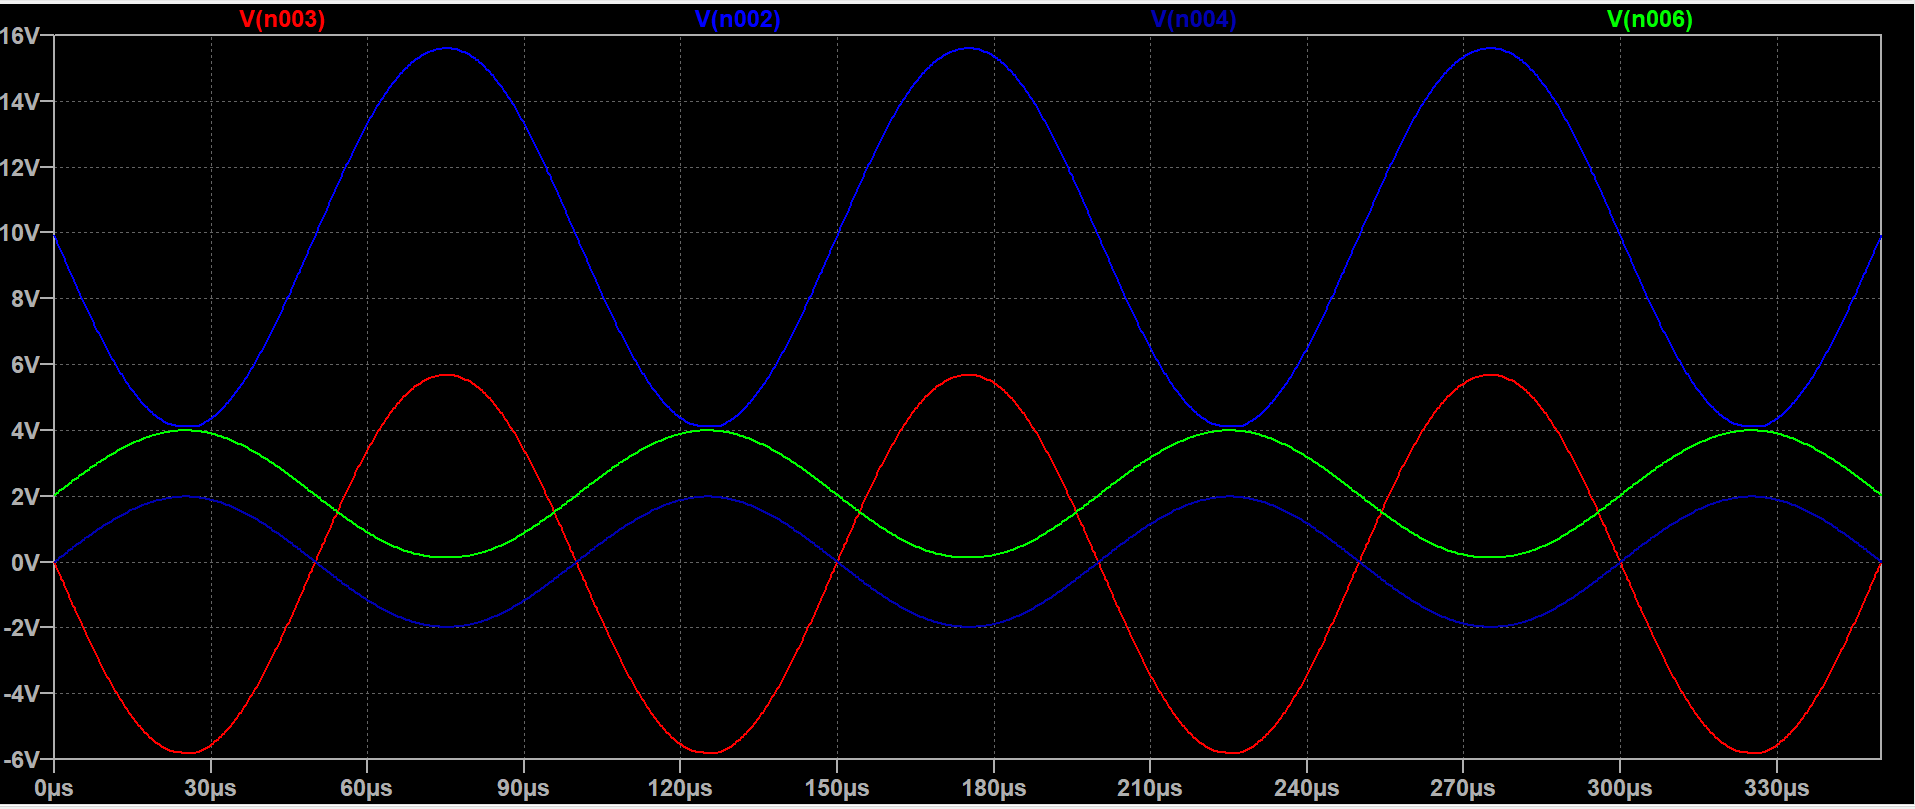
\includegraphics[scale=0.25]{sim4-2.png}
    \caption{$V_{\mathrm{AMP}} = 1.97\,\mathrm{V}$}
\end{figure}
\subsection{考察}
入力振幅 $0.5\,\mathrm{V}$ の場合には，
コレクタ電圧波形とエミッタ電圧波形の間に十分な差があり，
トランジスタが安定して動作していることが確認できる。
このとき，
コレクタ電圧波形は大きく変動しているのに対し，
エミッタ電圧波形の変動は比較的小さい。
そのため，
コレクタ・エミッタ間電圧 $V_{CE}$ に十分な余裕があり，
正常な増幅動作が行われていると考えられる。

一方，
入力振幅を $1.97\,\mathrm{V}$ まで増加させると，
コレクタ電圧波形の谷とエミッタ電圧波形の山が近づいていることが確認できる。
これは，
\[
V_{CE}=V_C-V_E
\]
が小さくなっていることを示しており，
トランジスタが正常な増幅領域の限界に近づいていると考えられる。






\section{実験5}
\subsection{実験内容}
1.で設定した動作点を左右にずらし、4.と同じ解析を行い、クリップ直前の出力波形を求め、
動作点との対応を考察した。
\subsection{結果}
はじめに、動作点を下図のように左に移動し、実験2と同様にして$R_A$と$R_B$を計算した。
\begin{figure}[H]
    \centering
    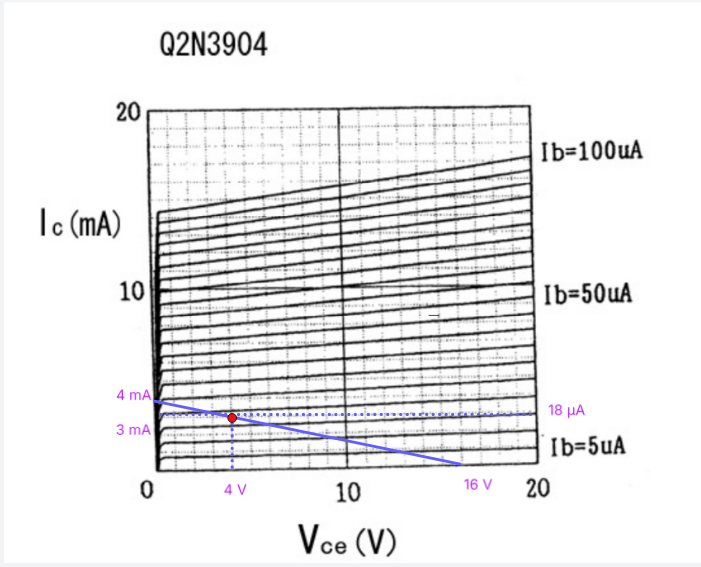
\includegraphics[scale=0.5]{hukatyokusenn5-1.png}
    \caption{動作点を左に移動したときの負荷直線}
\end{figure}
\[
R_A=\frac{V_{CC}-V_B}{I_1}
=\frac{16-3.65}{360\times10^{-6}}
\approx 34.306\,\mathrm{k\Omega}
\]
\[
R_B=\frac{V_B}{I_2}
=\frac{3.65}{342\times10^{-6}}
\approx 10.673\,\mathrm{k\Omega}
\]
これより、$V_{\mathrm{AMP}} = 0.5\,\mathrm{V}$のときと、クリップ直前のときの
回路図を以下に示す。
\begin{figure}[H]
    \centering
    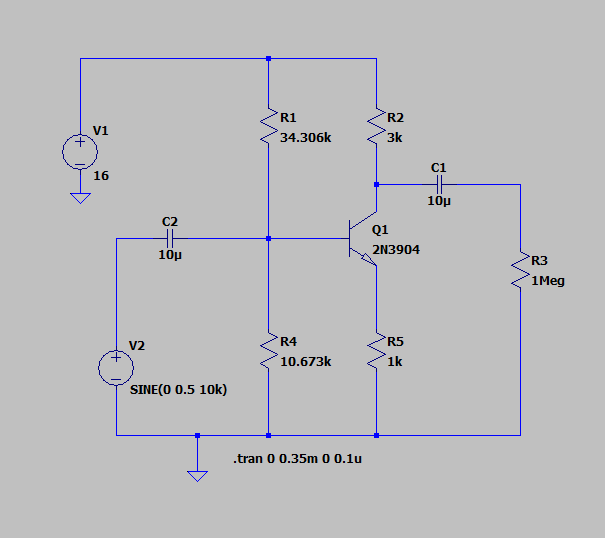
\includegraphics[scale=0.27]{kairozu5-1.png}
    \caption{$V_{\mathrm{AMP}} = 0.5\,\mathrm{V}$}
\end{figure}
\begin{figure}[H]
    \centering
    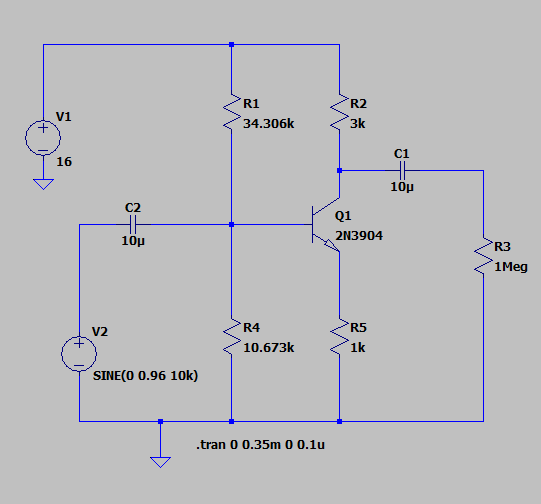
\includegraphics[scale=0.3]{kairozu5-2.png}
    \caption{$V_{\mathrm{AMP}} = 0.96\,\mathrm{V}$}
\end{figure}
以下にそれぞれの振幅における解析結果を示す。
ただし、黄色を入力波形、青色を出力波形、赤色をコレクタ電圧波形、紫色をエミッタ電圧波形
とする。
\begin{figure}[H]
    \centering
    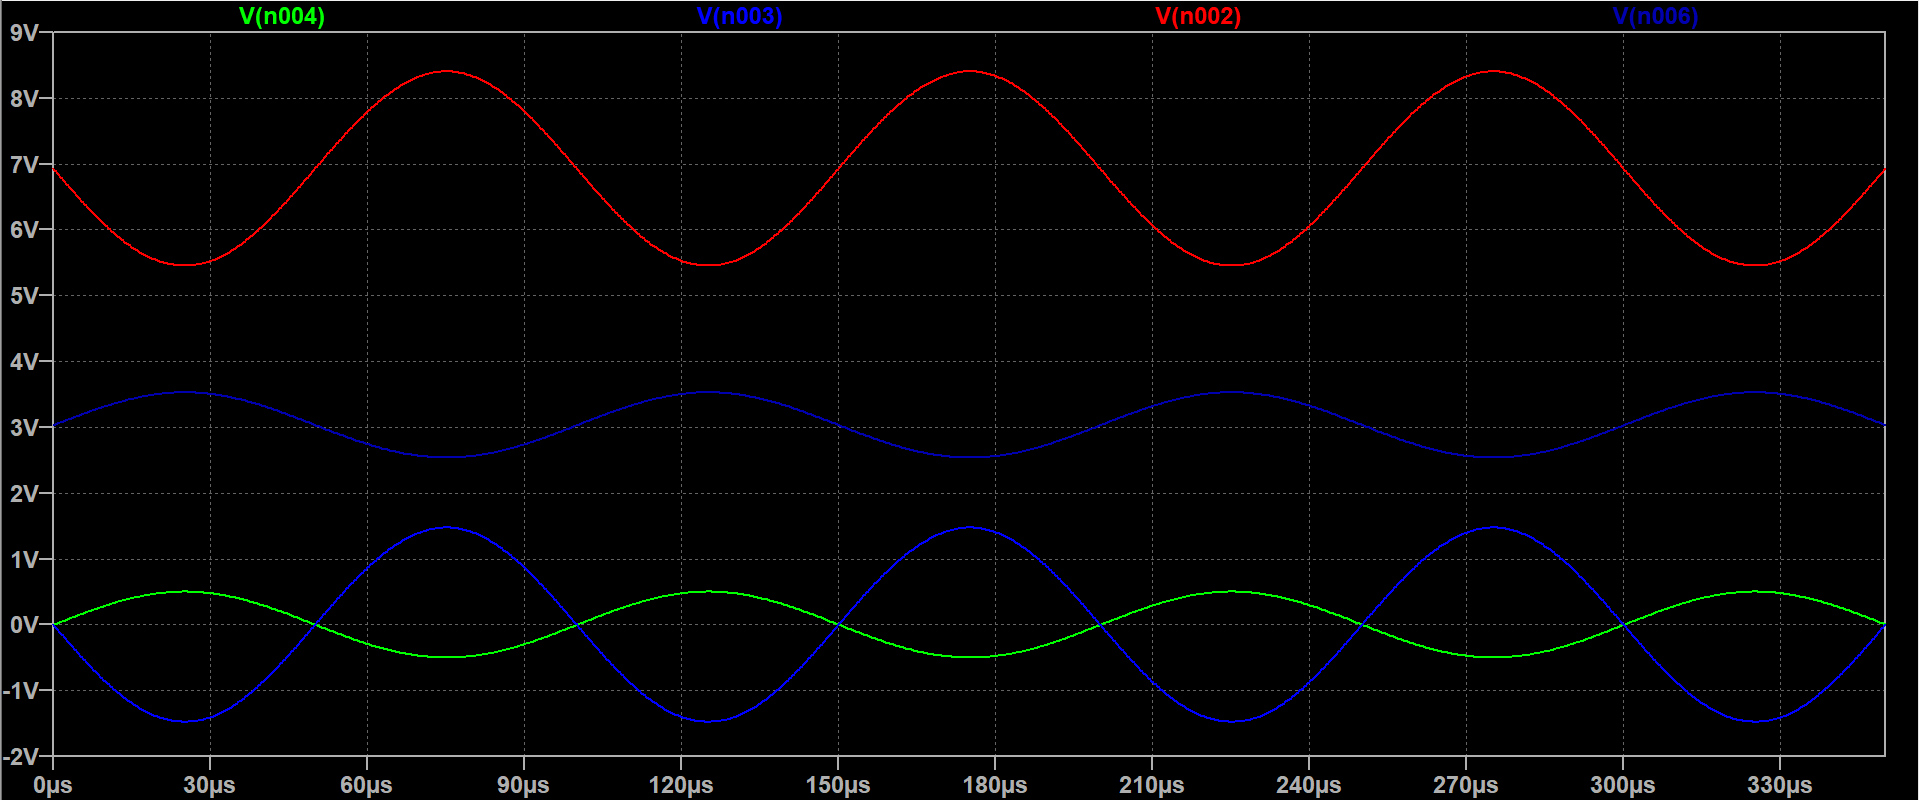
\includegraphics[scale=0.25]{sim5-1.png}
    \caption{$V_{\mathrm{AMP}} = 0.5\,\mathrm{V}$}
\end{figure}
\begin{figure}[H]
    \centering
    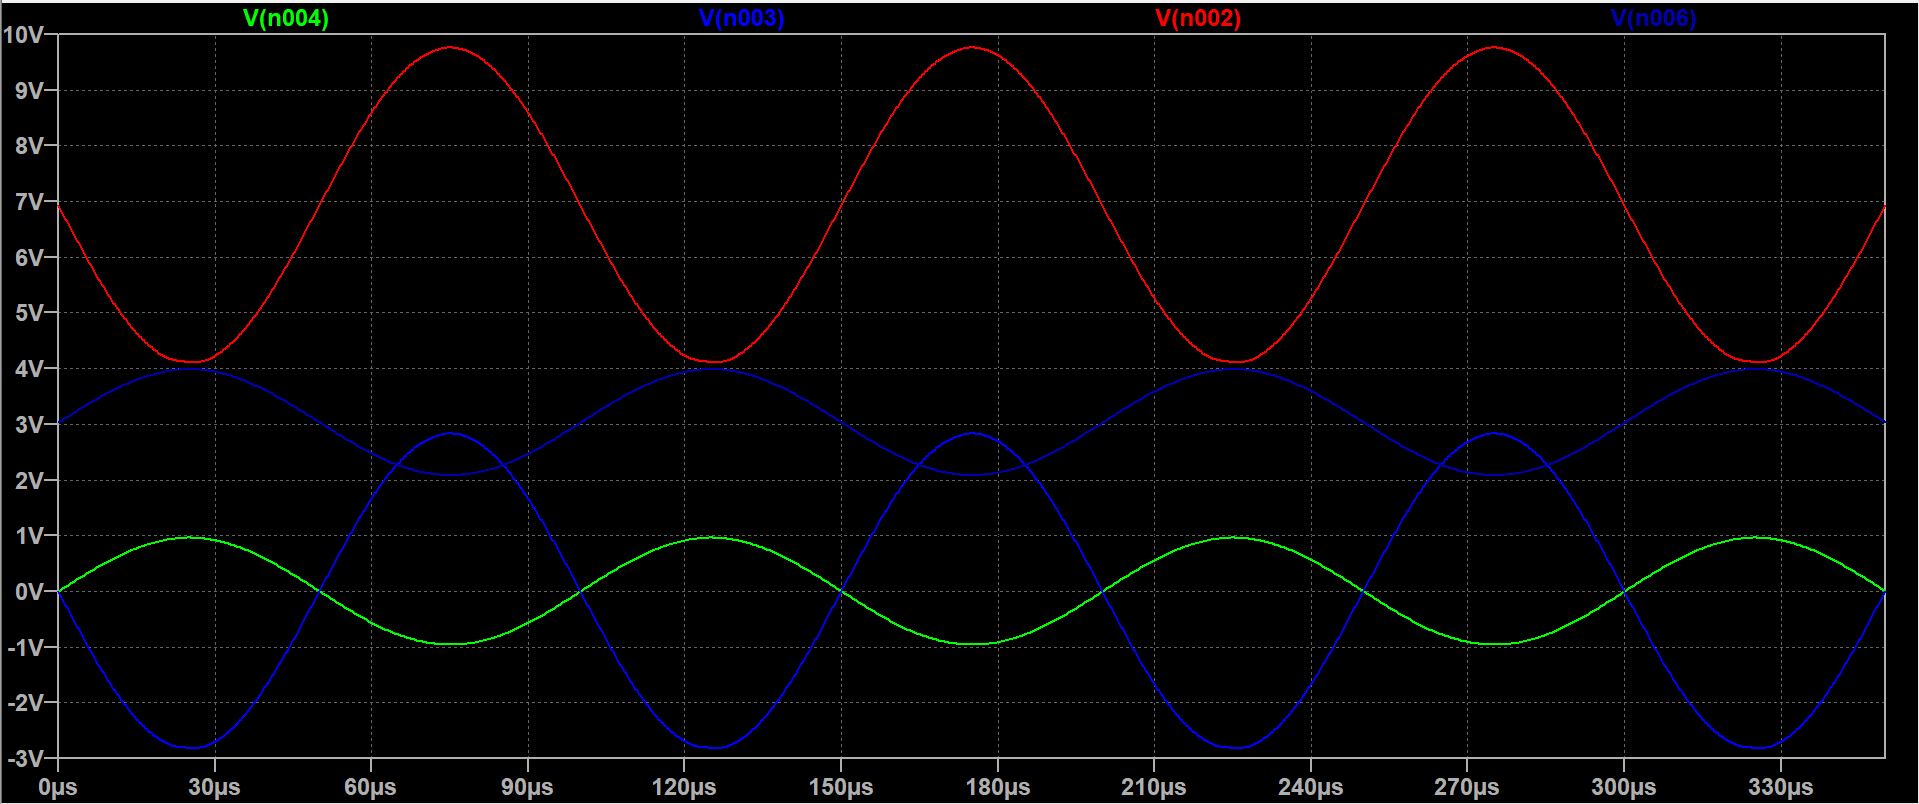
\includegraphics[scale=0.25]{sim5-2.png}
    \caption{$V_{\mathrm{AMP}} = 0.96\,\mathrm{V}$}
\end{figure}
次に、動作点を下図のように右に移動し、実験2と同様にして$R_A$と$R_B$を計算した。
\begin{figure}[H]
    \centering
    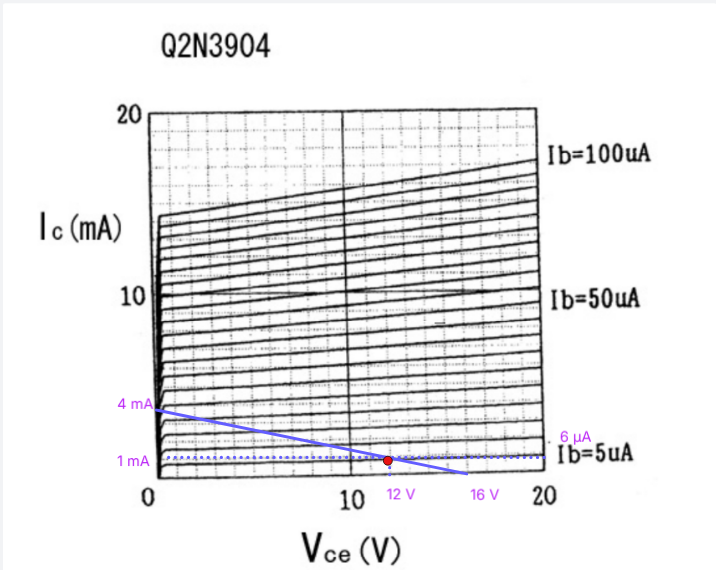
\includegraphics[scale=0.5]{hukatyokusenn5-2.png}
    \caption{動作点を右に移動したときの負荷直線}
\end{figure}

\[
R_A=\frac{V_{CC}-V_B}{I_1}
=\frac{16-1.65}{120\times10^{-6}}
\approx 119.58\,\mathrm{k\Omega}
\]
\[
R_B=\frac{V_B}{I_2}
=\frac{1.65}{114\times10^{-6}}
\approx 14.474\,\mathrm{k\Omega}
\]
これより、$V_{\mathrm{AMP}} = 0.5\,\mathrm{V}$のときと、クリップ直前のときの
回路図を以下に示す。
\begin{figure}[H]
    \centering
    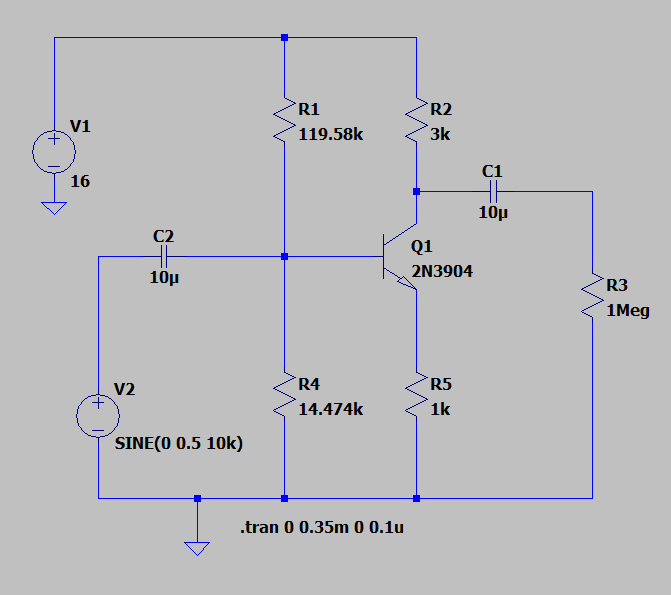
\includegraphics[scale=0.3]{kairozu5-3.png}
    \caption{$V_{\mathrm{AMP}} = 0.5\,\mathrm{V}$}
\end{figure}
\begin{figure}[H]
    \centering
    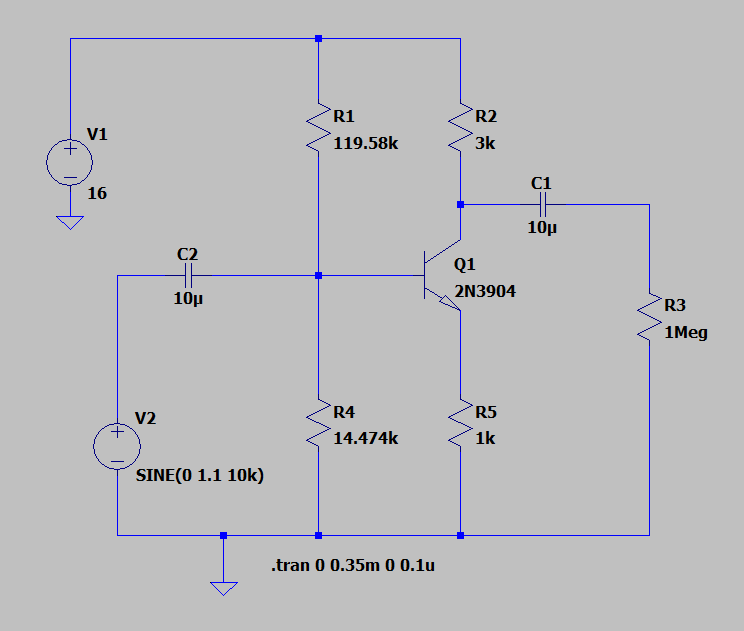
\includegraphics[scale=0.27]{kairozu5-4.png}
    \caption{$V_{\mathrm{AMP}} = 0.96\,\mathrm{V}$}
\end{figure}
以下にそれぞれの振幅における解析結果を示す。
\begin{figure}[H]
    \centering
    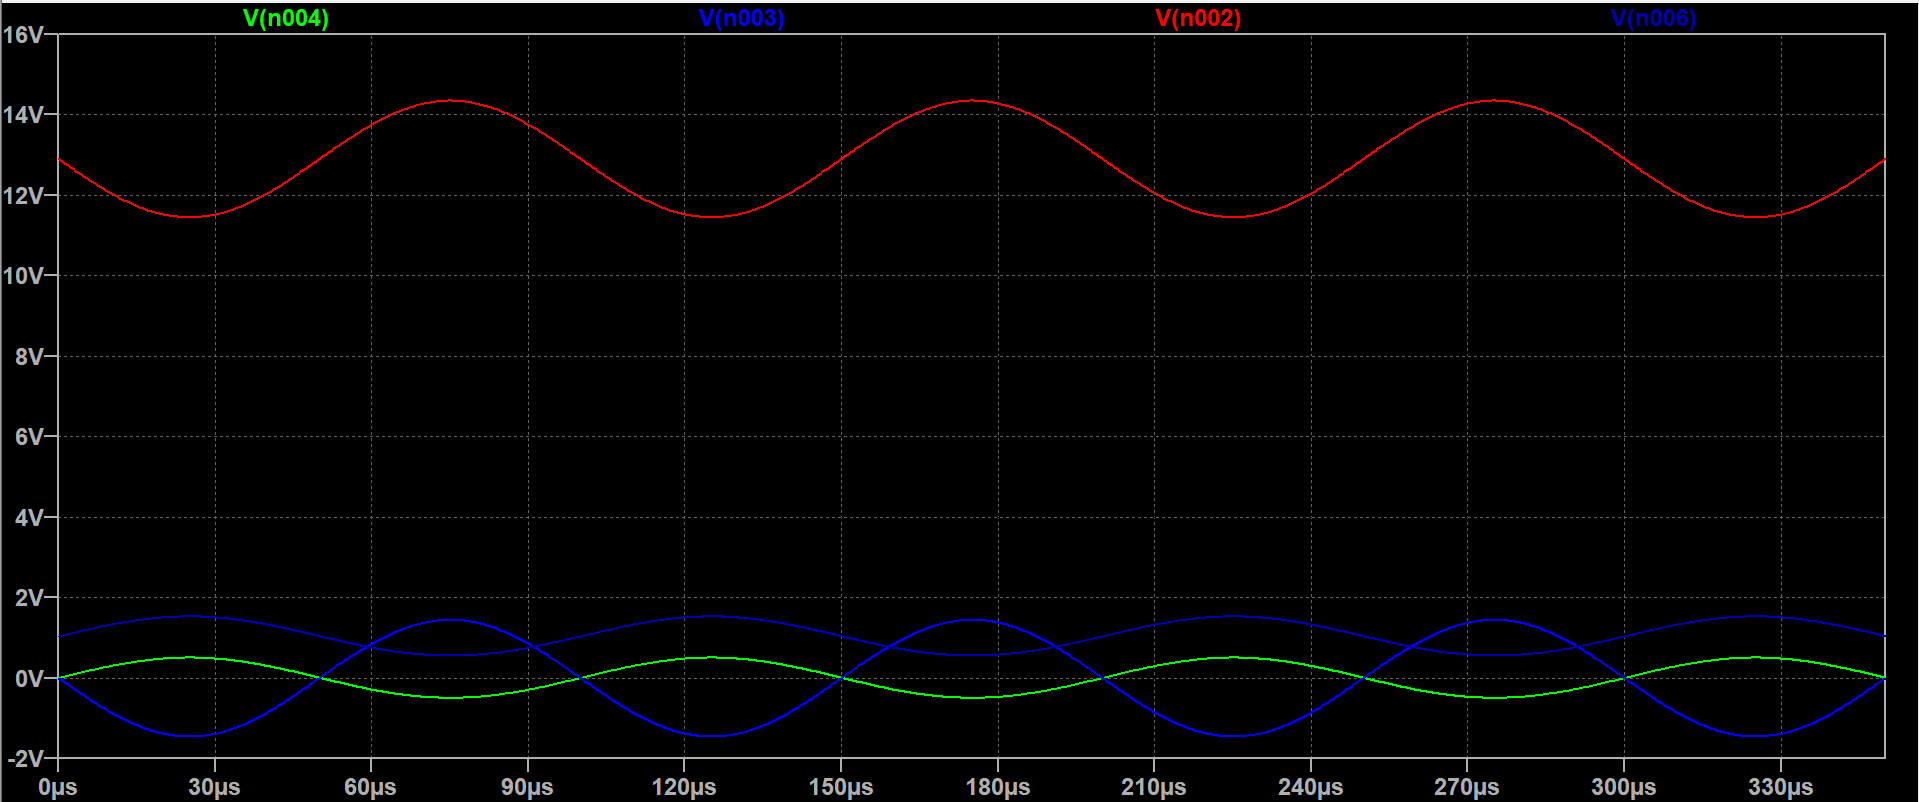
\includegraphics[scale=0.3]{sim5-3.png}
    \caption{$V_{\mathrm{AMP}} = 0.5\,\mathrm{V}$}
\end{figure}
\begin{figure}[H]
    \centering
    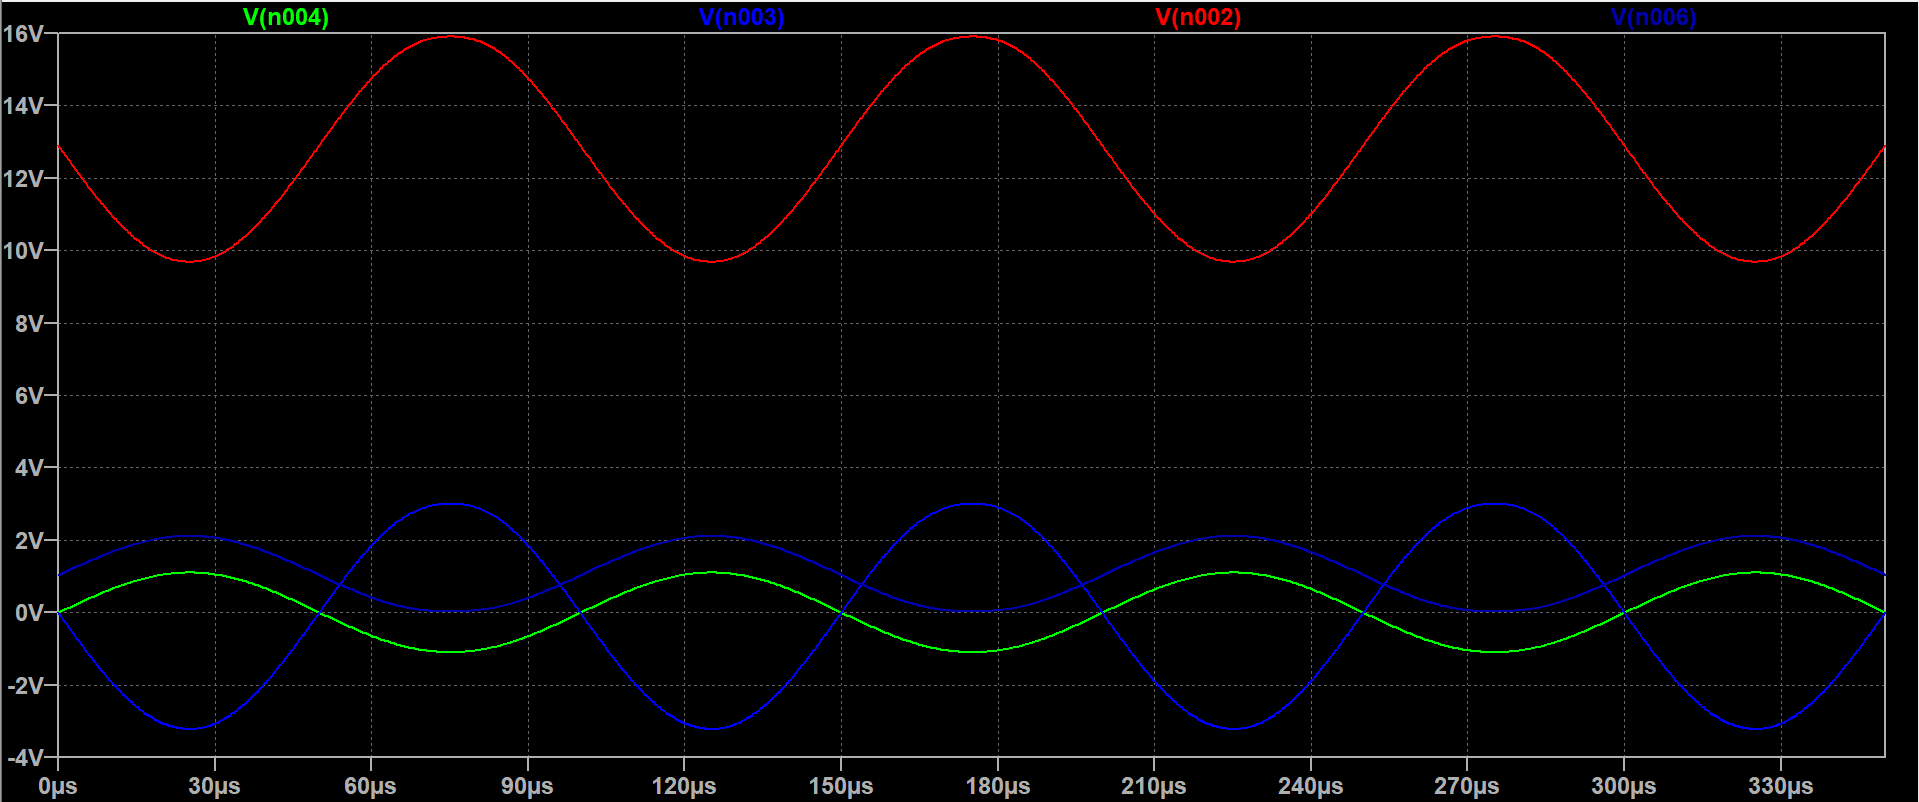
\includegraphics[scale=0.33]{sim5-4.png}
    \caption{$V_{\mathrm{AMP}} = 1.1\,\mathrm{V}$}
\end{figure}

\subsection{考察}

動作点を左側へ移動し、$V_{CE}=4\,\mathrm{V}$ とした場合、コレクタ電圧波形はおよそ
$
5.5\,\mathrm{V} \sim 8.4\,\mathrm{V}
$
の範囲で変動していた。
このとき、コレクタ電圧は低い電位付近で変動しており、上方向には
\[
16-8.4=7.6\,\mathrm{V}
\]
程度の余裕がある一方、下方向には約 $5.5\,\mathrm{V}$ 程度しか余裕がない。

また、コレクタ電圧波形の谷とエミッタ電圧波形の山が近づいていることから、
\[
V_{CE}=V_C-V_E
\]
が小さくなりやすい状態であることが分かる。
そのため、入力振幅を増加させると、コレクタ電圧が低電位側の限界へ早く近づき、動作可能範囲を超えやすくなると考えられる。
実際に、クリップ直前の入力振幅は約 $0.96\,\mathrm{V}$ となり、中央付近に動作点を設定した場合の約 $1.97\,\mathrm{V}$ と比較して小さくなった。

一方、動作点を右側へ移動し、$V_{CE}=12\,\mathrm{V}$ とした場合、コレクタ電圧波形はおよそ
$
11.5\,\mathrm{V} \sim 14.3\,\mathrm{V}
$
の範囲で変動していた。
この場合、下方向には約 $11.5\,\mathrm{V}$ の余裕があるが、上方向には
\[
16-14.3=1.7\,\mathrm{V}
\]
程度の余裕しかない。
したがって、入力振幅を増加させると、コレクタ電圧が高電位側の限界へ早く近づき、一方向に波形が歪みやすくなると考えられる。
実際に、クリップ直前の入力振幅は約 $1.1\,\mathrm{V}$ となり、中央付近の場合より小さくなった。

以上より、動作点を負荷直線の中央からずらすと、コレクタ電圧が変化できる範囲が一方向に偏るため、片側の限界へ早く到達し、出力波形がクリップしやすくなることが分かった。
したがって、動作点を負荷直線の中央付近に設定することは、出力波形の歪みを抑え、より大きな無歪出力を得るために重要である。


\section{感想}
今回の実験では、動作点を変化させることで出力波形の変化やクリップの発生の仕方が大きく変わることが分かった。
特に、動作点を負荷直線の中央付近に設定することが、波形の歪みを抑え、大きな無歪出力を得るために重要であることを確認できた。
また、周波数特性や時間域波形を実際に観察することで、トランジスタ増幅回路の動作原理への理解を深めることができた。
\end{document}




